\section*{Fragestellung}
Wie gut können Ionen und Moleküle in Lösungen detektiert werden und wie genau kann deren Konzentration bestimmt werden mit einem Selbstgebauten automatisiertem Prismenspektrograph?

\section*{Projektaufbau}
Der Prismenspektrograph besteht aus stationärer Optik, einem durch Stepper Motor bewegtem Photodetektor und Treiberelektronik.
Die stationäre Optik wird einmalig auf ein den sichtbaren Wellenlängenbereich kalibriert und in dieser Konfiguration festgeschraubt o.d.ä.
Der bewegliche Photodetektor wird entweder durch eine Raspberry Pi Kamera oder eine Photodiode realisiert die durch einen NEMA 17 Steppermotor hin und her bewegt wird um ein möglichst breites Spektrum genau abzudecken.
Bei Verwendung der Photodiode wird die Intensität über einen ADC von einem Arduino Uno gemessen und auf diesem direkt mit jeweiliger Stepperposition "verknüpft".
Bei Verwendung der Kamera geschieht die Bilderauswertung und Datenverknüpfung auf dem Raspberry Pi.

\begin{figure}[H]
    \centering
    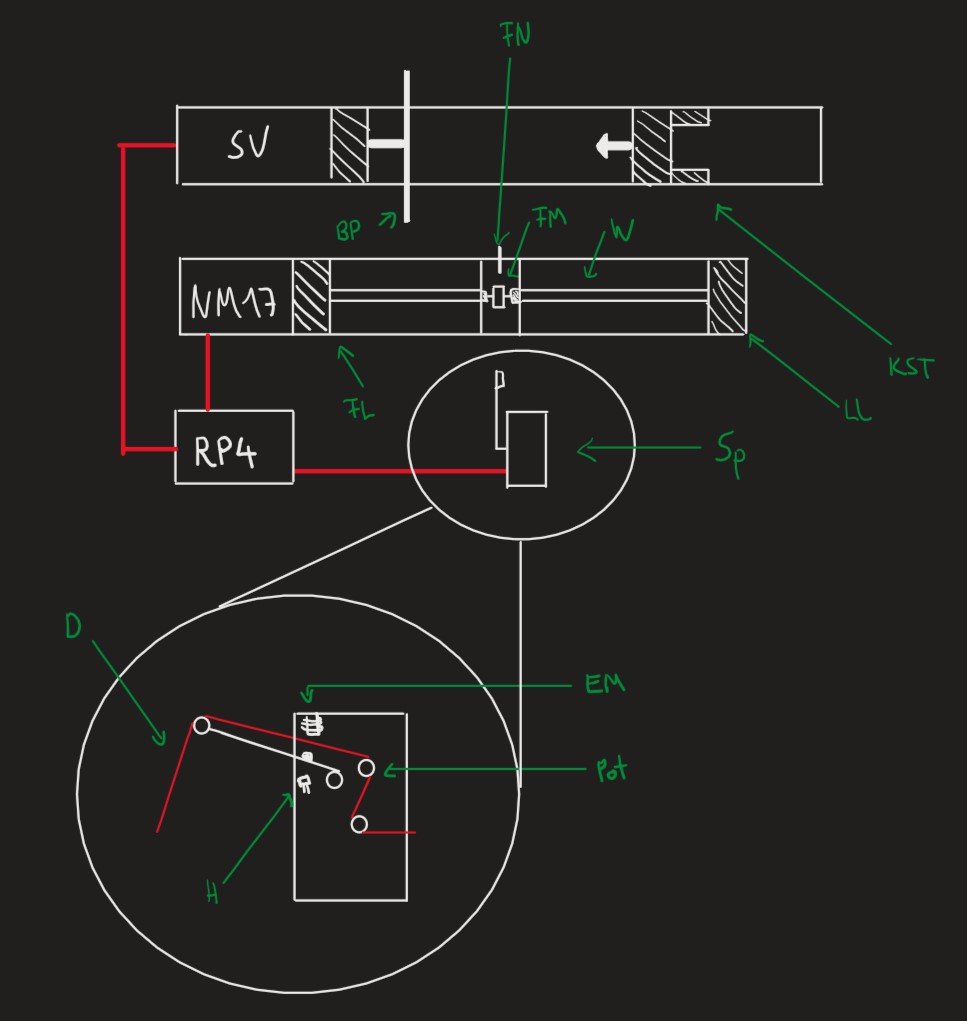
\includegraphics[width=\linewidth]{skizze.jpg}
    \caption{
        Skizze des Spektrographen mit Intensitätsaufnahme optional über Kamera oder Photodiode.
        \textbf{LQ}: Lichtquelle; 
        \textbf{L1,L2,K,F}: Linsen; 
        \textbf{O}: Untersuchungsobjekt; 
        \textbf{S}: Spalt; 
        \textbf{P}: Prismen; 
        \textbf{RP4}: Raspberry Pie 4 zur Datenanalyse; 
        \textbf{Kamera}: direkt an RP4; 
        \textbf{Photodiode}: über ADC an Arduino angeschlossen; 
        \textbf{NEMA 17}: Antrieb für Position der Kamera/Photodiode, über stepper driver an Arduino.
    }
    \label{fig:skizze}
\end{figure}


\section*{Physikalische Anforderungen}
\begin{enumerate}
    \item notwendiger Wellenlängenbereich der Photodiode ca. 300 - 800 nm.
    \item Dimensionen von der Wahl der Linsenbrennweiten abhängig.
    \item Optik muss genug Lichtintensität durchlassen um die Photodiode in einem möglichst linearem Bereich zu betreiben.
    \item Auflösungziel: $\Delta \lambda$ 0,5 nm.
\end{enumerate}


\section*{Komponenten und Kosten}
\begin{table}[H]
    \centering
    \caption{
        Skizze
    }
    \begin{tabular}{| c | c |}
        \hline
        Komponente &  Kosten / \euro{}\\
        \hline
        Linsen & 15 - 30  \\
        \hline
        Prismen & 15 - 30 \\
        \hline
        NEMA 17 & 8 - 15  \\
        \hline
        Stepper Driver & 6 - 10  \\
        \hline
        RP4 komp. Kamera & \quad 60 \\
        \hline
        Photodiode & 15 \quad  \\
        \hline
        sonst. Mat. & 50 - 80 \\
        \hline
        Arduino & vorhanden \\
        \hline
        RP4 & vorhanden \\
        \hline
        \hline
        Summe & 110 - 225  \\
        \hline
    \end{tabular}
    \label{tab:Komponenten}
\end{table}



\section*{Software}
\begin{enumerate}
    \item Stepper Steuerung und PhodotiodenIntensitätsmessung ($\mu$C)
    \item Telemetrie, Datenanalyse, Kalibration (RP4 C/C++ und Python)
\end{enumerate}

\section*{Aufwandsabschätzung}
\begin{table}[H]
    \centering
    \caption{
        Skizze
    }
    \begin{tabular}{| c | c |}
        \hline
        Arbeitspaket &  Aufwand / h\\
        \hline
        Optiktisch/Halterungen & 30 - 45  \\
        \hline
        Stepper Steuerung / ADC Messung & 10 - 15 \\
        \hline
        RP4 Telemetrie & 10 - 20  \\
        \hline
        RP4 Datenanalyse & 10 - 20  \\
        \hline
        Kalibration & 20 - 30 \\
        \hline
        Debugging & 50 - 100 \\
        \hline
        \hline
        Summe & 120 - 230  \\
        \hline
    \end{tabular}
    \label{tab:Aufwand}
\end{table}